\documentclass[a4paper,11pt,onecolumn,twoside]{ctexart}
\usepackage{amsmath,amssymb,amsfonts,amsthm,fancyhdr}
\usepackage{epsfig,graphicx,picins,picinpar,subfigure}
\usepackage{pstricks}
\usepackage{fancyvrb}
\usepackage[numbers,sort&compress]{natbib}
\usepackage{tikz}
\usepackage[linesnumbered, ruled, lined,boxed,commentsnumbered]{algorithm2e}[1]
\usepackage{caption}
\usepackage{graphicx}   % 导入图片
\usepackage{url}
\usepackage{hyperref}
\renewcommand{\theequation}{\arabic{section}.\arabic{equation}}
\renewcommand{\headrulewidth}{0.4pt}

\headsep=0.5truecm \footskip 0pt \topmargin 0pt \oddsidemargin 0pt
\evensidemargin 0pt \setlength{\textwidth}{14.8truecm}
\setlength{\textheight}{21.5truecm}
\setcounter{page}{1}
\pagestyle{fancy} \fancyhf{}
\hypersetup{colorlinks=false,pdfborder={0 0 0},}
\newtheorem{定理}{定理}[section]
\captionsetup[figure]{font=small}
\captionsetup[table]{font=small}

\makeatletter

\makeatother%用于连接公式编号

\begin{document}
	%------------------- 中文标题、作者、摘要和关键字
	
	\CTEXoptions[figurename={图}] \CTEXoptions[tablename={表}]
	\setlength{\columnwidth}{17.6cm}
	
	\title{{\Large \textbf{基于DFS的GaBP算法优化研究}}

	\footnotetext[1]{\zihao{-5}\textbf{收稿日期:} XXXX-XX-XX\quad
                \quad \quad \textbf{接受日期:} XXXX-XX-XX}
	\footnotetext[0]{\zihao{-5}\textbf{基金项目:}江苏省创新训练计划~(202410287190Y).}
	\footnotetext[0]{\zihao{-5}\textbf{作者简介:}邱德志(2004--), 男, 广西玉林, 本科生, 专业:信息与计算科学.\\ E-mail:082210219@nuaa.edu.cn.}
	\footnotetext[0]{\zihao{-5}\textbf{通讯作者:}陈思远(2004--), 男, 本科生, 专业:信息与计算科学.E-mail:misyun@nuaa.edu.cn}}
	
	\author{\zihao{5}邱德志~, 陈思远\\[-1pt]
	({\zihao{-5}南京航空航天大学 数学学院, 南京 210016})\\[-2pt]}
	

	
	\date{}
	\maketitle \vspace{-8mm}
	\thispagestyle{empty}
	\begin{center}  
		\begin{minipage}[c]{14cm}
			\zihao{-5} \mbox{}\hspace{2.4em}{\heiti 摘要:}\quad
			本文研究了 Gauss 信念传播算法在具有多个子系统的线性系统中的加速问题.利用深度优先遍历算法来减少 Gauss 信念传播算法在这一类线性系统中的计算复杂度,得到了DFS-GaBP算法.同时我们获得了DFS-GaBP算法在子系统上的收敛结果.我们的计算结果表明,对比传统算法,DFS-GaBP算法在具有多个子系统的线性系统中表现出更优的性能.\\
			\mbox{}\hspace{2.4em}{\heiti 关键词:}\quad Gauss信念传播算法,深度优先遍历,子系统,弱连通分量\\
			\mbox{}\hspace{2.4em}{\heiti MR(2010)主题分类号:}\quad 
			15A06 ; 65F10 \quad \quad \quad
			\mbox{}\hspace{2.4em}{\heiti 中图分类号:}\quad 
			O241.4  \\
			\mbox{}\hspace{2.4em}{\heiti 文献标识码: }\quad A
			\quad \quad \quad
			\mbox{}\hspace{2.4em}{\heiti 文章编号:}\quad \\

		\end{minipage}
	\end{center}
	\zihao{5}
	
	\vskip 0mm \noindent {\large {\bf 1 简介}} \vskip 3mm
	\setcounter{section}{1}\setcounter{equation}{0}
	
	线性数值代数的基本问题是求解一个线性方程组$Ax=b$,其中$A$为可逆矩阵,$b$是一个给定的向量.最初用来解决这类问题的基本方法是LU分解法(等价于Gauss消元法)和Cholesky分解法\cite{ref1}.这些方法通过将矩阵$A$分解为下三角矩阵$L$和上三角矩阵$U$(或对称正定矩阵的Cholesky分解),从而将原问题转化为两个易于求解的三角方程组.尽管直接法在理论上能够精确求解线性方程组,但当矩阵规模十分庞大且稀疏时,这些方法的计算复杂度和存储需求会显著增加,导致其在实际应用中效率低下.
	
	为了应对大规模稀疏线性方程组的求解问题,迭代算法应运而生.与直接法不同,迭代算法通过逐步逼近解的方式,能够在占用较少的计算资源的情况下获得近似解.经典的迭代算法包括Jacobi迭代法、Gauss Seidel迭代法\cite{ref2}以及共轭梯度法(Conjugate Gradient,CG)\cite{ref3}等.这些方法通过利用矩阵的稀疏性,显著降低了计算复杂度,特别适用于大规模问题的求解.然而,传统的迭代算法在某些情况下仍然存在收敛速度慢、对矩阵条件数敏感等问题,这促使研究者们不断探索更高效的算法.
	
	在本篇论文中,我们将探讨一种高效的分布式迭代算法——Gauss信念传播算法(Gaussian Belief Propagation, GaBP),用于求解线性方程组.GaBP 算法最初来源于概率图模型中的信念传播(Belief Propagation, BP)\cite{ref4}方法,其核心思想是将线性方程组的求解问题转化为特殊定义下的图上的概率推理问题.
	
	关于 GaBP 算法的基本属性,例如收敛性和计算复杂度,已有学者进行了深入研究.研究表明,原始的 GaBP 算法在矩阵$A$为对称正定且图结构为树图时能够稳定收敛\cite{ref5}.然而,这些条件在实际应用中往往过于严格,限制了算法的适用范围.例如,对称正定矩阵的要求意味着 GaBP 算法只能用于特定类型的线性方程组,而树图结构的限制则进一步缩小了其应用场景.
	
	在最近的研究中,有学者将算法进行了改进,将收敛条件进行了扩大,使得GaBP算法适用于非对称的线性系统\cite{ref6}.本论文将在此基础上进行讨论,运用数据结构中的相关知识,对一些具有特殊性质的矩阵在GaBP算法求解的运行过程下进行改良优化.
	
	深度优先搜索 (Depth-First Search, DFS)\cite{ref7} 是一种经典的图遍历算法, 广泛应用于图论、人工智能、网
	络分析以及组合优化等领域. 其核心思想是从一个起始节点出发, 沿着一条路径尽可能深入地访问节点, 直到
	无法继续深入为止, 然后回溯到上一个节点, 继续探索其他路径.DFS 通过递归或显式使用栈的方式实现, 能够
	系统地探索图或树的所有节点, 适用于解决路径查找、连通性检测、拓扑排序等问题.
	
	在实际应用中,DFS 被广泛用于多种场景.例如,在拓扑排序中,DFS 可以有效地对有向无环图(DAG)进行排序;在迷宫生成和求解中,DFS 可以生成随机的迷宫并找到从起点到终点的路径;在图的连通性检测中,DFS 可以判断图中是否存在从起点到终点的路径,或者找出所有的连通分量.此外,DFS 的变种如迭代加深 DFS(IDDFS)和双向 DFS 进一步扩展了其应用范围.IDDFS 通过限制搜索深度来避免 DFS 的深度过大问题,同时保留了 DFS 的空间效率;双向 DFS 则从起点和终点同时进行搜索,显著减少了搜索空间,适用于已知起点和终点的场景.
	
	本研究提出一种基于DFS的GaBP算法优化方法,通过系统性地整合DFS的图遍历特性与GaBP的消息传递机制,设计了一种改进的迭代流程,显著提升了算法在弱连通分量系统中的计算效率.
	
	在本文中,$I_n$为$n$阶的单位矩阵,
	$A^{T}$表示$A$的转置,
	$|A|$表示$A$的绝对值矩阵,
	$\rho(A)$表示$A$的谱半径,
	$\mathbf{diag}(A)$表示由方阵$A$的对角线元素构成的对角矩阵.
	假设$D$是对角矩阵,且对角元素非零,则$D^{-1/2}$表示将矩阵$D$的所有对角元素$d_{ii},(i=1,\cdots,n)$取为$1/\sqrt{d_{ii}}$得到的对角矩阵.
	
	\vskip 4mm \noindent {\large {\bf 2 基于DFS的GaBP}} \vskip 3mm
	\setcounter{section}{2}\setcounter{equation}{0}

	\noindent{\normalsize \bf 2.1 Gauss信念传播算法~~}\vskip 2mm

	信念传播算法最开始用于求解概率图模型中的边缘概率密度,后来Weiss等人经过研究发现其在Gauss图中的传播具有良好的特性,Bickson在2008年提出用于
	求解对称正定的线性系统的Gauss信念传播算法,2022年Fanaskov提出了用于非对称矩阵的GaBP算法.\cite{ref5,ref6,ref8}
	
	信念传播算法可以看作是概率图中每个顶点向周围发送信息的过程,给定每个节点的初始信息,我们要求每轮迭代中每个节点向邻接节点发送信息,这就是信念传播这一名称的由来.
	在树状图中,只要消息持续迭代下去,我们就一定能够得到每个节点的边缘概率密度,并且迭代次数等于树的直径.值得注意的是,在Gauss图中,每个节点的边缘概率密度可以由两个参数简单地进行表示:均值$\mu$和方差$\sigma^2$,这就意味着在Gauss图中使用信念传播算法,我们可以不用显式地去写出每个节点的概率密度,而只需要掌握每个节点的均值及方差即可,Gauss信念传播算法的迭代格式如下:
	\begin{equation} \label{GaBP的迭代格式}
		m_{ij}(x_j)\varpropto\int_{x_i}\psi_{ij}(x_i,x_j)\phi_i(x_i)\prod_{k\in N(i)\backslash j}m_{ki}(x_i)dx_i
	\end{equation}
	$m_{ij}(x_j)$表示节点$i$到节点$j$发送的消息,而$N(i)$表示节点$i$的所有邻接点的集合,其中自势函数$\phi_i$和边势函数$\psi_{ij}$的显式定义分别为$\phi_i(x_i)\triangleq \exp \left(-\frac{1}{2}A_{ii}x_i^2+b_ix_i\right)$,$\psi \triangleq \exp \left(-\frac{1}{2}x_iA_{ij}x_j\right)$.最终每个节点通过整合得到的消息,即可得到自身的边缘概率密度:
	\begin{equation} \label{边缘概率密度的迭代格式}
		p(x_i)=\alpha \phi_i(x_i)\prod_{k\in N(i)}m_{ji}(x_i)
	\end{equation}
	这里的$\alpha$为归一化参数.可以证明,在Gauss图中,所有传播的信息$m_{ij}(x_j)$以及自势函数$\phi_i(x_i)$都服从Gauss分布,因此只需保存每条信息的均值以及方差即可.为了更清楚地说明这一点,我们介绍下面的定理.
	
	{\bf 定理~2.1}~$^{[5]}$~~假设$X_1$与$X_2$分别为服从高斯分布的随机变量,$f_1(x)$与$f_2(x)$分别是$X_1,X_2$的概率密度函数,且$X_1\thicksim N(\mu_1,P_1^{-1}),X_2\thicksim N(\mu_2,P_2^{-1})$,那么$f(x)=f_1(x)f_2(x)$是分布为$N(\mu,P^{-1})$的随机变量的概率密度函数.其中
		\begin{align*}
			\mu&=P^{-1}(P_1\mu_1+P_2\mu_2)\\
			P^{-1}&=(P_1+P_2)^{-1}
		\end{align*}

	根据定理2.1,我们很容易就得到迭代格式(\ref{GaBP的迭代格式})的均值以及方差形式:
	\begin{equation} \label{GaBP的迭代格式的均值方差形式}
		P_{ij}^{(n+1)}=\overbrace{P_{ii}^{(n)}}^{\phi_i(x_i)}+\sum_{k\in N(i)\backslash j}\overbrace{P_{ki}^{(n)}}^{m_{ki}(x_i)},
		\mu_{ij}^{(n+1)}=\left(P_{ij}^{(n)}\right)^{-1}(\overbrace{P_{ii}^{(n)}\mu_{ii}^{(n)}}^{\phi_i(x_i)}+\sum_{k\in N(i)\backslash j}\overbrace{P_{ki}^{(n)}\mu_{ki}^{(n)}}^{m_{ki}(x_i)})
	\end{equation}
	对于(\ref{边缘概率密度的迭代格式})式同样可以写成均值以及方差的形式:
	\begin{equation} \label{GaBP的边缘概率密度的均值方差形式}
		P_i^{(n)}=\overbrace{P_{ii}^{(n)}}^{\phi_i(x_i)}+\sum_{k\in N(i)}\overbrace{P_{ki}^{(n)}}^{m_{ki}(x_i)},
		\mu_i^{(n)}=\left(P_i^{(n)}\right)^{-1}(\overbrace{P_{ii}^{(n)}\mu_{ii}^{(n)}}^{\phi_i(x_i)}+\sum_{k\in N(i)}\overbrace{P_{ki}^{(n)}\mu_{ki}^{(n)}}^{m_{ki}(x_i)})
	\end{equation}
	(\ref{GaBP的边缘概率密度的均值方差形式})式中的$\mu_i^{(n)},P_i^{(n)}$分别为第$n$次迭代得到的第$i$个边缘概率密度的均值与方差.上面的迭代算法被称为并行GaBP,其每一步的迭代都是使用上一轮迭代的结果.事实上GaBP算法可以使用本轮迭代的数据来进行迭代,这钟算法被称为串行GaBP.一般而言,串行GaBP的迭代速度要比并行GaBP的迭代速度更快,两者的关系类似于Jacobi迭代法和Gauss-Seidel迭代法.
	
	同时,GaBP算法也可以应对非对称线性系统,这时迭代格式变为:
	\begin{equation} \label{非对称GaBP的迭代格式}
		m_{ji}^{(n+1)}=P_{ji}^{(n)}\left(b_j+\sum_{k\in N_{in}(j)\backslash i}m_{kj}^{(n)}\right),P_{ji}^{(n)}=-\frac{A_{ij}}{A_{jj}+\sum_{k\in N_{in}(j)\backslash i}P_{kj}^{(n)}A_{kj}}\\
	\end{equation}
	\begin{equation} \label{非对称GaBP的边缘概率密度的迭代格式}
		\mu_{i}^{(n)}=\frac{b_i+\sum_{j\in N_{in}(i)}m_{ji}^{(n)}}{A_{ii}+\sum_{j\in N_{in}(i)}P_{ji}^{(n)}A_{ji}},P_{i}^{(n)}=A_{ii}+\sum_{j\in N_{in}(i)}P_{ji}^{(n)}A_{ji}
	\end{equation}
	其中$\mu_i^{(n)},P_i^{(n)}$即为计算得到的边缘概率分布的均值与方差,$N_{in}(i)\triangleq \{j|A(i,j)\neq 0\}$,同样地,我们可以定义$N_{out}(i)\triangleq \{j|A(j,i)\neq 0\}$,上面的迭代格式也同样可以改为串行格式.
	
	需要注意的是,(\ref{非对称GaBP的迭代格式})式与(\ref{非对称GaBP的边缘概率密度的迭代格式})式中的$m_{ji},P_{ij}$均为人为定义的消息,这是为了防止求解非对称线性系统的过程中出现的分母为$0$的情况.这点很容易理解,考察(\ref{GaBP的迭代格式的均值方差形式})式可以发现,由于$P$是协方差矩阵,因此是对称正定的,如果$P_{ij}^{(n)}$不为$0$,那么$P_{ji}^{(n)}$也同样不为零,但是在非对称线性系统中,该条件无法保证,因此要引入人为消息来避免这种情况发生(当然,在对称矩阵中,两类迭代格式是等价的).以上的GaBP算法都遵循定理3.1以及定理3.3的结论.
	\vskip 3mm\noindent{\normalsize \bf 2.2 线性系统的子系统~~}\vskip 2mm

	在介绍线性系统的子系统之前,我们首先给出图的基本术语.
	\begin{itemize}
		\item {\heiti 子图:}设有两个图$G=(V,E)$和$G'=(V',E')$,若$V'$是$V$的子集,且$E'$也是$E$的子集,则称$G'$是$G$的子图.
		\item {\heiti 连通图和连通分量:} 在无向图$G$中,若两个顶点之间存在路径,则认为这两个顶点是连通的.如果在无向图$G$中,任意两个顶点都是连通的,则称$G$是连通图.无向图中的极大连通子图被称为它的连通分量. 
		\item {\heiti 基图:} 将有向图的所有的有向边替换为无向边,所得到的图称为原图的基图.
		\item {\heiti 弱连通图和弱连通分量:} 假设有向图$G$的基图是连通图,则称$G$是弱连通图.有向图中的极大弱连通子图被称为它的弱连通分量.
	\end{itemize}
	
	由于GaBP可以视作在概率图中进行信息传播,因此我们可以从图的角度来进行思考:假设一个无向图可以被分为若干个连通分量,由于图中的每一个点都是由相邻点传播消息来得到
	该点的边缘概率密度,那么对其中的每一个点来说,处于不同连通分量的其它点不会对该点得到的信息产生影响,那么由此我们可以分别对不同的连通分量分别运行GaBP.
	为了说明这一点,我们考虑下面的无向图以及对应的邻接矩阵\footnote{这里的矩阵取自\cite{ref5}}:
	\begin{figure}[htbp] 
		\hspace*{-3cm}
		\centering
		\begin{minipage}{0.4\textwidth}
			%\centering
			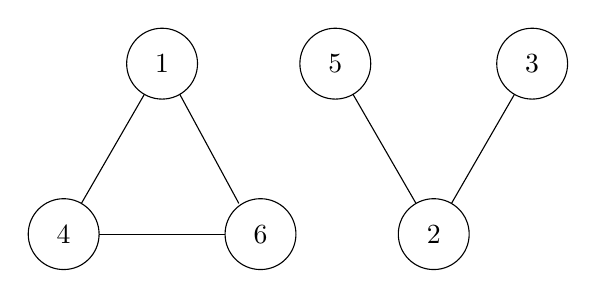
\begin{tikzpicture}
				\draw(0,0) circle [radius=0.45];
				\draw(2.5,0) circle [radius=0.45];
				\draw(1.25,2.165) circle [radius=0.45];
				\draw(0.45,0)--(2.05,0);
				\draw(0.225,0.3897)--(1.025,1.7753);
				\draw(1.475,1.7753)--(2.225,0.3897);
				\node[centered]at(0.0,0.0){4};
				\node[centered]at(2.5,0){6};
				\node[centered]at(1.25,2.165){1};
				
				\draw(4.7,0) circle [radius=0.45];
				\draw(3.45,2.165) circle [radius=0.45];
				\draw(5.95,2.165) circle [radius=0.45];
				\draw(4.475,0.3897)--(3.675,1.7753);
				\draw(4.925,0.3897)--(5.725,1.7753);
				\node[centered]at(4.7,0){2};
				\node[centered]at(3.45,2.165){5};
				\node[centered]at(5.95,2.165){3};
			\end{tikzpicture}
		\end{minipage}
		\begin{minipage}{0.4\textwidth}
			\hspace*{2cm}
			$
			\left(\begin{array}{cccccc}
				1&0&0&2&0&1\\
				0&1&-2&0&3&0\\
				0&-2&1&0&0&0\\
				2&0&0&2&0&1\\
				0&3&0&0&1&0\\
				3&0&0&1&0&1
			\end{array}\right)
			$
		\end{minipage}
		%\parbox{\dimexpr\linewidth-2cm}{\caption{一个具有两个连通分量的图以及对应的邻接矩阵}}
		\makebox[\linewidth]{\hspace{-3cm}\parbox{\dimexpr\linewidth-2cm}{\small \caption{一个具有两个连通分量的图以及对应的邻接矩阵}\label{两个连通分量的图和对应矩阵}}}
		
	\end{figure}
	上面的线性系统可以分成两个子系统,其中一个子系统由矩阵的第$1,4,6$行和列构成,记作$A\{1,4,6\}$,另外一个子系统由矩阵的第$2,3,5$行和列组成,记作$A\{2,3,5\}$.因此在求解线性系统时,我们可以将线性系统划分为若干个子系统分别求解,然后
	将得到的结果按顺序排列即可. 该方法具有以下优点:
	\begin{itemize}
		\item 可以减少GaBP的计算规模,我们从原先考虑的整体系统拆解为若干个子系统,子系统的规模要小于整体系统,从而减少计算量.
		\item 避免了计算冗余,在之前的算法中,我们通过遍历矩阵中的元素来考虑不同点之间是否会传播信息,在我们对系统进行拆解后,我们知道不同系统之间一定不会传播信息,这样就避免了不必要的计算.
		\item 不同子系统的性质不同,对于简单的子系统,我们能够使用更少的计算量来求解,从而将更多的计算资源给到颇具难度的系统中.
	\end{itemize}
	对于图1中的例子来说,由于$A\{2,3,5\}$所对应的无向图是直径为$3$的树图,因此对于任给的三维向量$b$,我们使用GaBP来求解线性系统$A\{2,3,5\}x=b$只需迭代$3$次.然而对于另外一个子系统$A\{1,4,6\}$,求解该系统所需的计算量
	要远大于$A\{2,3,5\}$,而$A\{2,3,5\}$在第三次迭代时就已经完成了收敛,所以在后续的计算中GaBP会产生计算冗余.如果将系统分开求解,我们就可以专注于还未收敛的系统,以此来减少计算量.
	\vskip 3mm\noindent{\normalsize \bf 2.3 深度优先遍历~~}\vskip 2mm
	由于拆分子系统可以提高GaBP的计算效率,因此我们可以使用DFS来寻找矩阵对应图中的所有子系统的结构.DFS可以利用邻接表或邻接矩阵来得到其对应无向图的所有连通分量,并输出连通分量上所有的点.该算法通过递归或显式使用栈的方式实现,DFS 的基本执行过程可以分为以下几个步骤:首先,选择一个起始节点并标记为已访问;然后,递归地访问其未访问的邻接节点.对于每个邻接节点,重复上述过程,直到当前路径上的所有节点都被访问完毕.当所有邻接节点都被访问后,算法回溯到上一个节点,继续探索其他未被访问的路径,当递归结束或栈为空时,表明当前的连通分量已经被访问过了,记录所有被访问的点
	,即为该连通分量上的所有点.此时寻找未被访问的点,重复上面的过程,直到所有的点都被访问.这样就能得到图中所有的连通分量以及其中的点.
	
	对于邻接表,DFS的计算复杂度为$O(V+E)$,对于邻接矩阵,两种算法的计算复杂度均为$O(V^2)$,而GaBP算法每次迭代的计算复杂度为$O(V^2)$,显然使用DFS寻找连通分量的代价是可接受的.因此我们考虑将DFS与GaBP相结合来求解线性系统.
	\vskip 3mm\noindent{\normalsize \bf 2.4 DFS-GaBP~~}\vskip 2mm
	考察非对称GaBP算法,我们注意到算法可以在弱连通分量中运行,因此在实际应用中,我们应该将图中所有的有向边变为无向边再应用DFS寻找连通分量,如果在矩阵中执行,可以做矩阵加法$B=|A|+|A^T|$,再对矩阵$B$执行DFS算法.通过对矩阵$B$执行DFS算法,我们能够得到矩阵$A$的所有子系统.
	
	对于$n$阶方阵$A$,假设$A$中所有子系统构成的集合为$\mathcal{S} (A)=\{A_1,A_2,\cdots,A_N\}$,$N$为弱连通分量的个数,通过DFS算法我们可以找到所有$A_i(i=1,\cdots,N)$的构造.每一次迭代分别在不同的$A_i$中执行GaBP算法,最终得到解向量$x=(x_1,x_2,\cdots,x_N)^T$,其中$x_i$是子系统$A_ix=b_i$的解.
	
	如果要求和原始GaBP算法的精确程度相当,
	那么DFS-GaBP算法的收敛阈值应不大于原始的GaBP,具体的收敛阈值需要根据实际情况具体选择.基于上面的考虑,我们正式定义了算法 \ref{算法1}.
	
	\SetKwInput{KwIn}{输入}
	\SetKwInput{KwOut}{输出}

	\SetAlCapFnt{\small} % 设置标题字体大小
	\SetAlCapNameFnt{\small} % 设置"Algorithm"字样字体
	\setlength{\algomargin}{1em} % 算法内容缩进(左右留白)

	\RestyleAlgo{ruled} % 保持带横线的样式
	\SetAlgoInsideSkip{0pt} % 减少算法内部间距


	\begin{algorithm}[H]
		
		%\SetAlgoNoLine
		\KwIn{系数矩阵$A$,向量$b$}
		\KwOut{解向量$x$}
		
		计算$B=|A|+|A^T|$,在$B$中执行DFS,得到子系统集合$\mathcal{S} (A)$.\\
		所有消息$m_{ij},P_{ij}$初始化为$0$,设置收敛阈值$\varepsilon$.\\
		\While{$\mathcal{S} (A)$不为空}
		{
			\For{$A_k\in \mathcal{S} (A)$}
			{
				\For{第$k$个连通分量$A_k$的第$i$节点$k_i$,令$m=b_{k_i},P=A_{k_{i}k_{i}}$.}
				{
					\For{$j\in N_{in}(k_i)$}
					{
						$m=m+\sum_{j\in N_{in}(k_i)}m_{jk_i}$,$P=P+\sum_{j\in N_{in}(k_i)}P_{jk_i}A_{jk_i}$
					}
					\For{$j\in N_{out}(k_i)$}
					{
						$P_{k_ij}=-A_{jk_i}/(P-P_{jk_i}A_{jk_i})$,$m_{k_ij}=P_{k_ij}(m-m_{jk_i})$
					}
					$x_{k_i}=m/P$
				}
				\If{解在$A_k$中收敛}
				{
					$\mathcal{S} (A)=\mathcal{S} (A)-\{A_k\}$
				}
			}
		}
		
		\caption{基于DFS的GaBP算法} \label{算法1}
		
	\end{algorithm}

	\vskip 4mm \noindent {\large {\bf 3 DFS-GaBP的性质}} \vskip 3mm
	\setcounter{section}{3}\setcounter{equation}{0}

	\noindent{\normalsize \bf 3.1 收敛性分析~~}\vskip 2mm

	关于GaBP的收敛性有来自Malioutov等人\cite{ref9}的结果,我们可以利用其结果来分析DFS-GaBP算法.
	对于线性系统$Ax=b$,假设矩阵可以分为若干个子系统,则存在排列方阵$P$,使得
	\begin{equation} \label{A与对角块的关系}
		P^TAP=
		\left(
		\begin{array}{cccc}
			A_1&&& \\
			&A_2&& \\
			&&\ddots&\\
			&&&A_k
		\end{array}
		\right)\triangleq \varLambda 
	\end{equation}
	显然$\varLambda$是准对角矩阵,这时线性问题转化为$\varLambda Px=Pb$.由于$P$是排列矩阵,因此它仅仅只重新排列矩阵的行和列,而不
	改变矩阵元素的数值,所以我们有如下结论.

	\vskip 1mm{\bf 定理~3.1}~~矩阵$A$对角占优当且仅当矩阵$\varLambda$对角占优.
	
	首先\cite{ref8}中提出当矩阵可逆且对角占优时,GaBP算法收敛.而根据定理3.1,我们知道矩阵$A$收敛时所有的子矩阵$A_i$都是对角占优的.实际上
	DFS-GaBP的过程是在每一个$A_i$上分别执行GaBP算法,由于DFS算法可以寻找每个弱连通分量具有哪些节点,因此我们可以省去寻找排列矩阵$P$的过程.
	而所有的$A_i$都是对角占优的,因此GaBP在所有的$A_i$上收敛,基于上面的分析我们可以得到DFS-GaBP收敛的充分条件.
	\vskip 1mm{\bf 定理~3.2}~~矩阵$A$可逆且对角占优时,DFS-GaBP收敛.
	
	上面的定理在实际上比较实用,因为矩阵的对角性质较为容易判断.而在理论上,关于GaBP的收敛性有更加一般的结论.
	
	\vskip 1mm{\bf 定理~3.3}~$^{[9]}$~~假设矩阵$A$满足条件
		\begin{equation}
			\rho(|I_n-D^{-1/2}AD^{-1/2}|)<1
		\end{equation}
	则GaBP收敛,其中$D=\mathbf{diag}(A)$.
		
	但当矩阵$A$满足定理3.3的条件时,$\varLambda$的对角块矩阵是否满足相同的条件?事实上,答案是肯定的,并且这是一个充要条件.因此
	当矩阵$A$满足上述的条件时,所有的$A_i$满足一样的条件,于是DFS-GaBP在每个$A_i$上收敛.
	
	\vskip 1mm{\bf 定理~3.4}~~当矩阵$A$满足条件
		\begin{equation}
			\rho(|I_n-D^{-1/2}AD^{-1/2}|)<1
		\end{equation}
		则GaBP在每一个$A_i$上收敛,即DFS-GaBP收敛,其中$D=\mathbf{diag}(A)$.

		{\bf 证} 事实上,由于每个$A_i$都是$\varLambda$上的对角块矩阵,因此我们只需要证明
		\begin{equation}
			\rho(|I_n-D^{-1/2}AD^{-1/2}|)<1 \Leftrightarrow \rho(|I_n-S^{-1/2}\varLambda S^{-1/2}|)<1
		\end{equation}
		即可,其中$S=diag(\varLambda)$.根据(\ref{A与对角块的关系})式,其中的$P$是排列矩阵,因此也同时是正交矩阵,得到
		\begin{align*}
			D^{-1/2}AD^{-1/2}&=D^{-1/2}P\varLambda P^TD^{-1/2}\\
			&=(PP^T)D^{-1/2}P\varLambda P^TD^{-1/2}(PP^{T})\\
			&=P(P^TD^{-1/2}P)\varLambda (P^TD^{-1/2}P)P^{T}
		\end{align*}
		因为$(P^TD^{-1/2}P)\varLambda (P^{T}D^{-1/2}P)=P^TD^{-1/2}AD^{-1/2}P$,而$D^{-1/2}AD^{-1/2}$对角线上元素均为$1$,$P$为排列矩阵,因此
		矩阵$(P^TD^{-1/2}P)\varLambda (P^{T}D^{-1/2}P)$的对角线元素均为$1$,容易验证$P^TD^{-1/2}P$是对角矩阵,因此$P^TD^{-1/2}P=S^{-1/2}$.
		则有$D^{-1/2}AD^{-1/2}=PS^{-1/2}\varLambda S^{-1/2}P^T$.于是
		\begin{align*}
			I_n-D^{-1/2}AD^{-1/2}&=I_n-PS^{-1/2}\varLambda S^{-1/2}P^T\\
			&=PP^T-PS^{-1/2}\varLambda S^{-1/2}P^T\\
			&=P(I_n-S^{-1/2}\varLambda S^{-1/2})P^T
		\end{align*}
		由于$P$是排列矩阵,而对于矩阵$A$,取绝对值和行列交换两种操作是可交换的.因此有$|PAP^T|=P|A|P^T$,所以根据上面的式子,我们有
		$|I_n-D^{-1/2}AD^{-1/2}|=P|I_n-S^{-1/2}\varLambda S^{-1/2}|P^T$,于是$|I_n-D^{-1/2}AD^{-1/2}|$和$|I_n-S^{-1/2}\varLambda S^{-1/2}|$等价,
		这样就证明了$\rho(|I_n-D^{-1/2}AD^{-1/2}|)<1 \Leftrightarrow \rho(|I_n-S^{-1/2}\varLambda S^{-1/2}|)<1$.
	
	我们还可以证明定理3.4的条件是定理3.2的条件的充分条件,因此定理3.4的条件更加一般.而在实际应用中我们更
	多地使用定理3.2.
	\vskip 3mm\noindent{\normalsize \bf 3.2 时间复杂度分析~~}\vskip 2mm	
	\begin{table} 
		\begin{center}
			\makebox[\linewidth]{\hspace{-3cm}\parbox{\dimexpr\linewidth-2cm}{\caption{算法时间复杂度比较}}}
			\hspace*{-3cm}
			\begin{tabular}{|p{2cm}|p{5cm}|}
				\hline
				算法&时间复杂度\\
				\hline
				GaBP&$k\times O(n^2)$\\
				\hline
				DFS-GaBP&$O(n^2)+\sum_{A_i\in \mathcal{S} (A)}k_i\times O(n_i^2)$\\
				\hline
			\end{tabular}
		\end{center}
	\end{table}
	假设矩阵$A$的阶数为$n,A$的弱连通分量的集合为$\mathcal{S} (A)=\{A_1,A_2,\cdots,A_k\}$,分别记弱连通分量的节点个数分别为$n_i(i=1,\cdots,k)$.根据($\ref{A与对角块的关系}$)式,我们
	知道DFS-GaBP每次迭代的时间复杂度为:$\sum_{i=1}^{k}O(n_i^2)$,由于$\sum_{i=1}^{k}n_i=n$,因此一定有$\sum_{i=1}^{k}n_i^2\leqslant n^2$,而GaBP每次迭代的时间复杂度为$O(n^2)$,因此
	在理论上DFS-GaBP每次迭代的计算量要少于原始GaBP.表1比较了两者的时间复杂度.
	
	在实际应用中,可仅对未收敛的弱连通分量执行GaBP.如果GaBP算法在其中某个子系统$A_k$中收敛了,那么接下来的计算中我们不需要在$A_k$中进行迭代,这时$\mathcal{S} (A)=\mathcal{S} (A)-\{A_k\}$,因此实际上每次迭代时间复杂度应该为$\sum_{A_i\in \mathcal{S} (A)}O(n_i^2)$.由于执行DFS的计算复杂度为$O(n^2)$,这与原始GaBP算法每次迭代
	的计算量相当,所以在有多个子系统的线性系统中,我们可以使用DFS-GaBP算法来求解线性方程组.
	
	\vskip 4mm \noindent {\large {\bf 4 实验及其分析}} \vskip 3mm
	\setcounter{section}{4}\setcounter{equation}{0}
	
	\noindent{\normalsize \bf 4.1 基于黑油模型的 IMPES 模拟矩阵~~}\vskip 2mm
	
	图2是一个油藏模拟的5005阶稀疏矩阵\cite{ref10}的零元素比例分块热图以及连通分量热图,右图中不同颜色代表着不同的连通分量,我们使用DFS算法计算得到该矩阵具有2111个连通分量.
	
	\begin{figure}[htbp]
		\hspace*{-3cm}
		\centering
		\includegraphics[scale=0.4]{零元素比例分块热图2}
		\includegraphics[scale=0.4]{主热图}
		\makebox[\linewidth]{\hspace{-3cm}\parbox{\dimexpr\linewidth-2cm}{\caption{矩阵结构及其连通分量热图}}}
	\end{figure}
	
	
	我们以该矩阵为基础,以$10^{-5}$为收敛阈值使用了Jacobi迭代、SOR迭代、GMRES子空间法(最大迭代步长为20000)、原始GaBP算法以及我们改进之后的DFS-GaBP算法进行了求解和比较,并记录了它的迭代情况和各算法计算时间情况如下:
	
	
	\begin{figure}[htbp]
		\hspace*{-3cm}
		\centering
		\includegraphics[scale=0.4]{5005迭代3}
		\includegraphics[scale=0.4]{5005时间}
		
		\makebox[\linewidth]{\hspace{-3cm}\parbox{\dimexpr\linewidth-2cm}{\caption{迭代次数(纵坐标为$\| \mathbf{x}^{(n)} - \mathbf{x}^{(n-1)} \|_2$)以及算法计算时间比较}}}
	\end{figure}
	
	
	
	在这一算法中,我们首先看到Jacobi迭代的速度十分缓慢,迭代曲线十分平缓,迭代了57304次才成功收敛.另外GMRES子空间法无法适用于这个问题,算法无法收敛.而SOR迭代法则表现较好,GaBP算法与DFS-GaBP算法也稳步收敛.
	
	再通过计算时间的比较我们可以更好的发现DFS-GaBP的优势所在(此处因GMRES子空间法无法收敛所以取了一个较大值).在所有算法中,只有SOR迭代法和DFS-GaBP算法对这个问题有十分优秀的计算效率,而DFS-GaBP算法是计算时间最少,也就是计算效率最高的算法.通过比较,我们也发现DFS-GaBP算法计算该问题的时间,比原始GaBP算法快了将近八倍,取得了较好的成果.
	\vskip 3mm\noindent{\normalsize \bf 4.2 化学过程模拟矩阵~~}\vskip 2mm	
	我们继续在一个21982阶的化学模拟矩阵\cite{ref11}上进行实验,该矩阵具有11091个连通分量,且是对角占优矩阵,但该矩阵不可逆,因此我们只增加矩阵对角线元素的值,不改变其结构的情况下使其可逆.由于子空间法在该矩阵上很难收敛,因此我们只使用GaBP算法与迭代法来进行求解.结果如图4所示.
	
	\begin{figure}[h]
		\hspace*{-3cm}
		\centering
		\includegraphics[scale=0.4]{11091迭代曲线}
		\includegraphics[scale=0.4]{11091收敛时间}
		\makebox[\linewidth]{\hspace{-3cm}\parbox{\dimexpr\linewidth-2cm}{\caption{迭代次数(纵坐标为$\| \mathbf{x}^{(n)} - \mathbf{x}^{(n-1)} \|_2$)以及算法计算时间比较}}}
	\end{figure}
	
	在这个矩阵中,通过收敛曲线我们可以发现GaBP算法的迭代速度较快,但计算时间长,但是对于DFS-GaBP算法而言,其收敛曲线与GaBP算法相当,但是计算时间比其他所有算法都要少,因此在这一线性系统中,我们的算法仍然是最优的.
	\vskip 3mm\noindent{\normalsize \bf 4.3 随机构造的修正矩阵~~}\vskip 2mm
	我们运用程序自带的随机生成指令,构造出一个1000阶且连通分量为562个的稀疏矩阵,其零元素比例分块热图如下:
	\begin{figure}[h]
		\hspace*{-3cm}
		\centering
		\includegraphics[scale=0.4]{构造的热图}
	\end{figure}
	
	将这个1000阶的矩阵同样以$10^{-5}$为收敛阈值使用Jacobi迭代、SOR迭代、GMRES子空间法(最大迭代步长为20000)、原始GaBP算法以及我们改进之后的DFS-GaBP算法来进行求解比较,所得的计算结果如下:
	
	\begin{figure}[h]
		\hspace*{-3cm}
		\centering
		\includegraphics[scale=0.4]{构造迭代}
		\includegraphics[scale=0.4]{构造时间}
		\makebox[\linewidth]{\hspace{-3cm}\parbox{\dimexpr\linewidth-2cm}{\caption{迭代次数(纵坐标为$\| \mathbf{x}^{(n)} - \mathbf{x}^{(n-1)} \|_2$)以及算法计算时间比较}}}
	\end{figure}
	
	我们发现DFS-GaBP在这个矩阵中的表现情况无疑也是非常好的,与GaBP一样,经过较少的迭代次数就很快地接近我们的收敛阈值.而且计算时间同样也是在这些算法中最少的.
	
	通过上述几个实验我们发现,在线性系统具有多个子系统的情况下,DFS-GaBP算法的计算效率是优于原始GaBP算法的.所以在处理大规模矩阵中,比起GaBP算法,DFS-GaBP算法的表现更好.
	
	\vskip 4mm \noindent {\large {\bf 5 总结}} \vskip 3mm
	GaBP算法在求解大型稀疏矩阵上要优于传统的迭代法,而DFS-GaBP算法在处理具有多个子系统的线性系统上具有一定的优势,同时执行DFS所需要的计算量是可以被接受的.我们证明了当整体系统满足收敛条件时,所有的子系统也同样满足收敛条件,因此可以在所有的子系统上应用GaBP算法.并且我们选取了几个较大规模的矩阵来验证我们算法的性质,可以看到DFS-GaBP算法和GaBP算法在
	这些系统中的收敛性质相当,并且我们优化后的算法每次迭代所需的计算量要少于原始的GaBP算法.
	
	
	\begin{thebibliography}{0}
		\bibitem{ref1}徐树方, 高立, 张平文. 数值线性代数(第2版)[M]. 北京: 北京大学出版社, 2013.
		\bibitem{ref2}郝艳花. Jacobi迭代法与Gauss-Seidel迭代法[J]. 山西大同大学学报(自然科学版), 2017, 33(05):3-5.
		\bibitem{ref3}何国良, 张文星, 赵熙乐. 共轭梯度法的直观解释[J]. 大学数学, 2022, 38(01): 73-82.
		\bibitem{ref4}郑汉垣. 大规模稀疏线性方程组求解的并行GaBP算法研究[D]. 上海: 上海大学, 2014.
		\bibitem{ref5}Bickson D. Gaussian Belief Propagation: Theory and Application[D]. Jerusalem: The Hebrew University of Jerusalem, 2009.
		\bibitem{ref6}Fanaskov V. Gaussian belief propagation solvers for nonsymmetric systems of linear equations[J]. SIAM Journal on Scientific Computing, 2022, 44(1): A77-A102.
		\bibitem{ref7}孙涵, 黄元元, 高航, 等. 数据结构: 抽象建模、实现与应用[M]. 北京: 机械工业出版社. 2020.
		\bibitem{ref8}Weiss Y, Freeman W T. Correctness of Belief Propagation in Gaussian Graphical Models of Arbitrary Topology[J]. Neural Computation, 2001, 13(10): 2173-2200.
		\bibitem{ref9}Malioutov D M, Johnson J K, Willsky A S. Walk-Sums and Belief Propagation in Gaussian Graphical Models[J]. Journal of Machine Learning Research, 2006, 7: 2031-2064.
		\bibitem{ref10}Sherman A. Oil reservoir simulation challenge matrices IMPES simulation of a black oil model[DB/OL]. \url{https://math.nist.gov/MatrixMarket/data/HarwellBoeing/sherman/sherman3.html}, 1984.
		\bibitem{ref11}Velzen N V. Chemical process simulation[DB/OL]. \url{https://sparse.tamu.edu/VanVelzen/std1\_Jac3\_db}, 2006.
		
		
	\end{thebibliography}
	
		\newcommand{\engtitle}{\zihao{-3}\bfseries Research on Optimization of GaBP Algorithm Based on DFS}
	\newcommand{\engauthor}{
		\zihao{-4} \textit{Qiu Dezhi, Chen Siyuan} \\
		\zihao{-5} (College of Mechanical and Electrical Engineering, Nanjing University of Aeronautics \& Astronautics, Nanjing 210016, China)
	}
	
	
	
	\begin{center}
	\Large\textbf{Research on Optimization of GaBP Algorithm Based on DFS} \\[6pt]
	\author{\zihao{5}{Qiu Dezhi,  Chen Siyuan}\\[-1pt]
	(\textit{\zihao{-5} School of Mathematics, Nanjing University of Aeronautics \& Astronautics, Nanjing 210016, China })
	}
	\end{center}
	
	\begin{center}
		\mbox{}\hspace{2.3em}\textbf{Abstract: } {\small This paper investigates the acceleration of the Gaussian belief propagation (GaBP) algorithm in linear systems with multiple subsystems. By utilizing a depth-first search (DFS) algorithm to reduce the computational complexity of the GaBP algorithm in such linear systems, we obtain the DFS-GaBP algorithm. Meanwhile, we derive convergence results for the DFS-GaBP algorithm on the subsystems. Our computational results demonstrate that, compared to traditional algorithms, the DFS-GaBP algorithm exhibits superior performance in linear systems with multiple subsystems.}\\ 
		\mbox{}\hspace{2.3em}\textbf{Keywords:}\quad Gaussian Belief Propagation,Depth-First Search,Subsystem,Weak connected components
	\end{center}
	

\end{document}